\chapter{Obecný popis metody}
\setcounter{page}{1}
\pagenumbering{arabic}

V této kapitole popíšeme základní koncept naší metody. Detailní popis zmíněných
dvou částí, které jsou stěžejními tématy této práce, bude následovat v dalších
dvou kapitolách. Naše metoda je založena na řízeném iterativním pohybu ligandu
skrze tunel, díky čemuž se vyhneme časově náročnému výpočtu stochastického
pohybu ligandu, který je typický pro simulace molekulární dynamiky.

Prvním krokem naší metody je diskretizace tunelu jejímž výstupem je posloupnost
omezujících podmínek, díky kterým můžeme definovat pozici ligandu v tunelu a
tím pádem i směr jeho pohyb tunelem – dopředu a dozadu. Na takto diskretizovaném
tunelu je poté ligand iterativně dokován na sérii po sobě jdoucích pozic v tunelu,
což nám umožňuje simulovat proces navázání ligandu nebo naopak jeho uvolnění.





\section{Diskretizace tunelu}
K tomu abychom mohli s ligandem tunelem iterativně procházet, potřebujeme nějakým
způsobem omezit prostor, ve kterém může být ligand umístěn.
Omezení se v našem případě realizuje pomocí posloupnosti koulí, které aproximují
geometrii tunelu. Takovouto aproximaci můžeme získat například pomocí nástroje
Caver \cite{Caver}. Na vstupu algoritmu tedy máme zmíněnou posloupnost
koulí, kterou náš algoritmus transformuje na posloupnost $ n $ řezů - kruhů
$ \theta_1, \dots, \theta_n $. Tyto řezy generujeme tak, abychom tunel rozdělili
na pláty, které mají shora omezenou tloušťku (to proto abychom nevynucovali
příliš velké změny v pozici ligandu mezi jednotlivými kroky výpočtu). Prakticky
se jedná o 2D kruhy, které omezují prostor, na který můžeme ligand zadokovat.
Cestu ligandu tunelem pak definujeme jako posloupnost umístění vybraného atomu
ligandu na po sobě jdoucí řezy (výběr atomu je libovolný, ale musí být stejný
pro všechny řezy). Popis algoritmu pro diskretizaci tunelu je obsahem první kapitoly.

\begin{figure}[t]
\centering
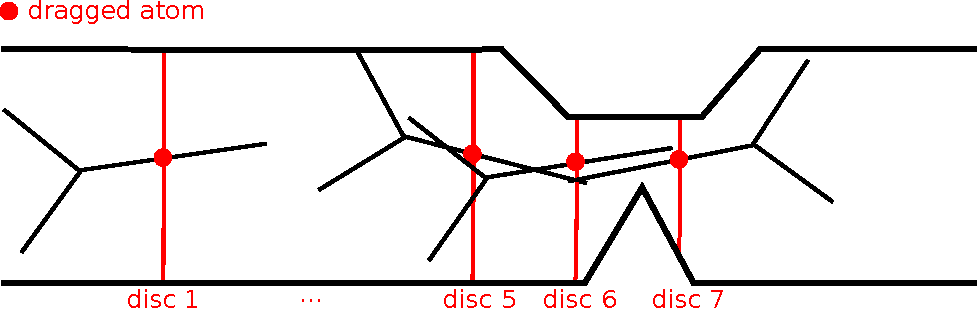
\includegraphics[width=.8\hsize]{img/tun.pdf}
\caption{Schématický 2D pohled na průchod tunelem. Vybraný atom ligandu je
postupně umisťován na po sobě jdoucí disky. Tím že nezajišťujeme spojitý pohyb
ligandu, můžeme vidět, že mezi řezy $\theta_6$ a $\theta_7$ dochází k prudké rotaci, v
důsledku čehož nedetekujeme úzké a potenciálně neprůchodné hrdlo tunelu.}
\label{fig:lower-bound}
\end{figure}





\section{Doking s omezujícími podmínkami}
Konformace ligandu $ \lambda $ je definována pozicí atomů
$ \lambda = \{a_i\}^m_{i = 1} $ v klasické kartézské souřadné soustavě. Maje
k dispozici diskretizaci tunelu, můžeme vybrat atom ligandu $ a_c \in \lambda $,
a poté iterativně provádět doking ligandu na disky $ \theta_1, \dots, \theta_n $,
přičemž budeme požadovat, aby výsledná konformace ligandu po dokingu na
$ i $-tý disk splňovala $ a_c \in \theta_i $. Tímto způsobem ligand přinutíme
k tomu, aby prošel celým tunelem.

Trajektorie ligandu vygenerovaná tímto způsobem navzorkuje profil tunelu bez
výraznějších mezer (to znamená, že ligand nebude schopen překonat (přeskočit) například
úzká hrdla tunelu), nicméně problémem je, že nemusí být spojitá (ligand se
může mezi sousedními řezy volně rotovat). Tuto nespojitou trajektorii budeme
používat jakožto dolní odhad na transportní energii. Příklad takové trajektorie
je vykreslen na obrázku č. \ref{fig:lower-bound}. Jak můžeme vidět, atom $ a_c $
je přichycen ke kruhu a jeho posunem skrze tunel modelujeme transportní
proces. Na obrázku lze také vidět příklad nespojitého pohybu – konkrétně
se jedná o otočení ligandu mezi řezy $ \theta_7$ a $\theta_8$.

Spojitou trajektorii můžeme vypočítat tak, že při přechodu mezi po sobě jdoucími
řezy omezíme pohyb každého z atomů na nějaké jeho $ \delta $– okolí. Přesněji řečeno
budeme požadovat, aby vzdálenost atomů v nové konformaci ligandu $ \lambda^{i + 1} $
od příslušných atomů v předchozí konformaci $ \lambda^{i} $ byla shora omezená
konstantou $ \delta > 0 $. Formálně
\begin{align}
    a_j \in \lambda^{i}, b_j \in \lambda^{i + 1} \Rightarrow |a_j - b_j| < \delta.
    \label{eq:pattern}
\end{align}

\begin{defi} \label{def:strong_pattern}
V této situaci řekneme, že $ \lambda^i $ je vzorem omezujícím konformaci
$ \lambda^{i+1} $ a budeme značit $ \lambda^{i+1} \in \Delta \lambda^i $ jestliže
je splněna podmínka (\ref{eq:pattern}).
\end{defi}


\begin{figure}[t]
\centering
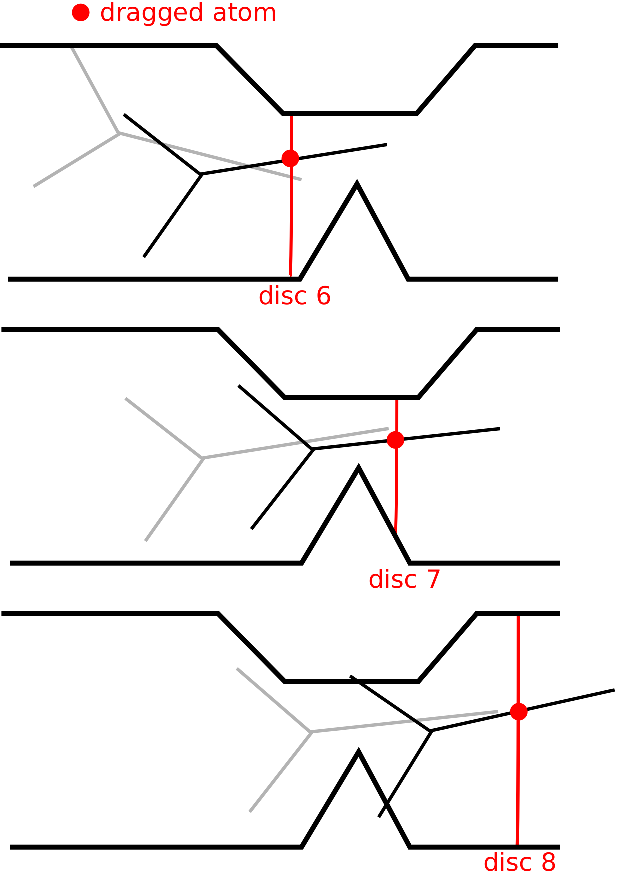
\includegraphics[width=.5\hsize]{img/tun-2.pdf}
\caption{Schématický 2D pohled na průchod tunelem, při kterém je předchozí pozice
ligandu použita jakožto omezující vzor. Omezení pohybu atomů zapříčiní, že geometrické
úzké hrdlo mezi řezy $\theta_6$ a $\theta_7$ je detekováno, neboť ligand nyní
nemá možnost rotace. Ve výsledném energetickém profilu bychom pak viděli prudké
zvýšení energetického potenciálu v místě zadokování ligandu na řez č. 8.}
\label{fig:continuous_transition}
\end{figure}

V průběhu výpočtu pak kdykoliv počítáme další konformaci $ \lambda^{i+1} $,
omezíme pohyb ligandu na aktuální vzor $ \lambda^{i} $. Díky tomu budeme mít
garantováno, že $ \lambda^{i+1} \in \Delta \lambda^i $, z čehož plyne, že
transformace konformací ligandu mezi po sobě jdoucími řezy bude spojitá
(shora omezená kladnou konstantou $ \delta $). Na tomto místě musíme poznamenat, že aby
výše uvedený postup dával smysl, musí platit, že každé dva po sobě jdoucí řezy jsou
od sebe vzdáleny o vzdálenost menší než $ \delta $. Demonstraci použití
omezujícího vzoru můžeme vidět na obrázku č. \ref{fig:continuous_transition}. Jak
vidno omezující vzor nedovolí ligandu rotaci jakou jsme mohli pozorovat
v předchozím případě (obrázek č. \ref{fig:lower-bound}), což nám umožní detekovat
úzké geometrické hrdlo.





\section{Hledání minimální spojité trajektorie}
Iterativním dokováním za použití výše popsaného omezení na konformační vzor můžeme
získat spojitou trajektorii. Našim cílem ovšem bude najít trajektorii, jejíž
celková energie bude co nejmenší. Z tohoto důvodu chceme ligandu
umožnit optimalizovat jeho pozici na každém z disků tak, aby jeho potenciální
energie byla co nejmenší. Toto minimum ale již po první iteraci nemusí být dostupné
kvůli omezením, které na atomy ligandu klade omezující vzor. Proto na každém
z řezů $ \theta_i $ budeme pro výchozí konformaci $ \lambda^i_j $ hledat dílčí
trajektorii (spojitou transformaci ligandu) $ \lambda^i_{j+1} \in \Delta \lambda^i_j,
\lambda^i_{j+2} \in \Delta \lambda^i_{j+1}, \dots $, která ve výsledku
zlepší potenciální energii ligandu oproti jeho výchozí konformaci $ \lambda^i_j $.
Tyto kroky budeme nazývat optimalizační kroky, neboť umožňují ligandu transformaci
do nízkoenergetické konformace, která ihned po přechodu z $ \theta_{i - 1} $
na $ \theta_i $ nemusí být dosažitelná.

\begin{figure}[t]
\centering
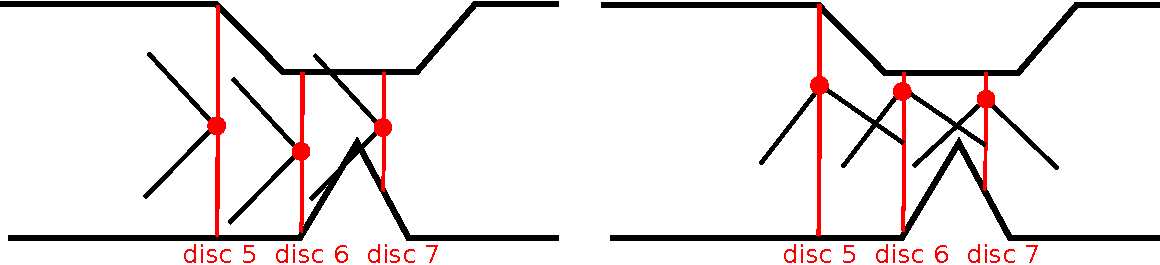
\includegraphics[width=.8\hsize]{img/tun-3.pdf}
\caption{Srovnání průchodu ligandu tunelem, při kterém se zasekne (vlevo) a
průchodu s alternativní výchozí konformací, díky které se ligandu podaří
úzké hrdlo překonat (vpravo).
}
\label{fig:backtracking}
\end{figure}

Výše uvedený postup bude obecně preferovat pohyb ligandu, který vede ve směru
největšího energetického gradientu. Ačkoliv je takový scénář v reálné situaci
nejpravděpodobnější, může se také stát, že dojde k posunu ligandu do nějaké
jiné konformace, která mu může pomoci překonat energetickou bariéru, která se
vyskytuje v tunelu někde dále. Uvažme například situaci na obrázku
č. \ref{fig:lower-bound}. V závislosti na výchozí orientaci ligand úzké hrdlo
může, ale také nemusí překonat. Kvůli tomu musíme začít uvažovat vícero potenciálních
trajektorií.

Počet všech možných spojitých trajektorií je velmi vysoký – roste exponenciálně vzhledem
k počtu řezů: přechod na následující disk může změnit pozici ligandu, orientaci
nebo konformaci (relativní pozici atomů v rámci ligandu). Vyčerpávající zkoušení
všech možných trajektorií tedy nepřipadá v úvahu vzhledem k tomu, že čas
potřebný k zadokování ligandu s omezeními se obvykle pohybuje mezi stovkami
milisekund až sekundami. Kvůli tomu jsme byli nuceni zavést jednoduchou heuristiku:
pokud je potenciální energie pozice $ \lambda^i_j $ významně větší než potenciální
energie nějaké již známé konformace $ \lambda^i_{low} $ (například konformace
získaná během výpočtu dolního odhadu na energii trajektorie), nastavíme
$ \lambda^i_j = \lambda^i_{low} $ a začneme prohledávat tunel z tohoto místa
směrem dozadu přes řezy $ \theta_{i-1}, \theta_{i-2}, \dots $. Backtracking
skončí ve chvíli, kdy dojde ke konvergenci dopředné a zpětné trajektorie a jsou
navázány nebo v případě, že se dostaneme na úplný začátek tunelu.
Algoritmus pro detekci konvergence trajektorií je obsahem druhé kapitoly.

